\chapter{Case Study: Building Certified Sequential OS Kernels}
\label{chap:seq:kernel}
\ignore{\section{Overview of Certified Sequential Kernels}}
To demonstrate the power of our new languages and tools,
we have applied our new layered approach to specify and
verify four variants of sequential \mCTOS{} kernels in the Coq proof assistant.
This Chapter presents how to verify  these kernels as a case study and the benefits of our layered approach.

The \mCTOSbase{} base kernel is a simplified uniprocessor version of
the CertiKOS kernel~\cite{gu11} designed for the 32 bit x86
architecture.  It provides a multi-process environment for user-space
applications using separate virtual address space, where the
communications between different applications are established by
message passing.  The \mCTOShyper{} kernel, built on top of the base
kernel, is a realistic hypervisor kernel that can boot recent versions
of unmodified Linux operating systems (Debian 6.0.6 and Ubuntu
12.04.2).  The \mCTOSringz{} kernel extends the hypervisor supporting
``ring 0'' processes, hosting ``certifiably safe'' services and
application programs inside the kernel address space.  Finally, we
strip the last kernel down to the \mCTOSembed{} kernel, removing
virtualization, virtual memory, and user-space interrupt handling.
This results in a minimal operating system suitable for embedded
environments.

This Chapter is organized as below:
In Section~\ref{sec:seq:design}, we present
our principles to introduce new layers.
Section~\ref{sec:seq:base} shows
how to build certified layers for  a sequential kernel
\mCTOS{}.
Based on this one,
Section~\ref{sec:seq:extend}
describes how to build variants of different sequential
kernels in our layered approach.

%\sectskip
\section{Principles for Layer Design}
\label{sec:seq:design}
%\asectskip

Our layered framework  provides an elegant formalism for decomposing
the verification of a complex kernel into a large number of tractable
tasks: we design a series of certified abstraction layers, which serve
as increasingly deep specifications for an increasing portion
of the kernel code.  These abstract layers are designed in a way such
that complex interdependent kernel components are untangled and
converted into a well-organized kernel-object stack with clean
specification.  In this section, we present the layer design process
and common principles we have followed in our development.


\paragraph{Principle 1: introduce layers to reflect dependencies between kernel modules} One purpose 
of layers is to enforce code isolation and abstraction.
When a module $M$ depends on another module $N$,  
abstraction layers should be organized in such a way that
$M$ can be reasoned about in terms of an abstracted version of $N$.

For example, since the virtual memory management code relies on physical memory management,
the code which performs allocation and
deallocation of physical pages in terms of allocation tables
is first abstracted into a layer object (\cf Figures~\ref{fig:alt}-\ref{fig:palloc:spec}).
This object provides the primitives \code{palloc} and \code{pfree} to operate on an abstract allocation
table \code{AT}.
Then functions such as \code{pt\_insert} and \code{ pt\_rmv}, which manipulate
page mappings at the virtual memory management level,
can be verified with a more
abstract view of the allocation
table, without worrying about its concrete memory representation and code
implementation.
On the other hand, if two kernel modules mutually depend on each other,
they have to be introduced within a single layer.

\ignore{
\paragraph{Principle 2: introduce a layer when the abstraction of kernel object changes}
(I am not sure whether this principle should be explicitly listed here or not -- Ronghui)

[Speculation by jeremie, try and add examples:]
On occasion,
it might be useful to offer multiple views of a single kernel object
at different levels of abstraction.
For instance,
in cases where there is a very large gap between
the concrete data structures used by a layer object and
the abstract description we ultimately want to use,
it can be simpler to decompose the refinement proof in two steps
by introducing an intermediate representation
which is already somewhat abstracted,
but similar in structure to the concrete implementation.
More over,
client code in different parts of the kernel
might be better understood with different levels of abstraction
for their kernel object. [Is that true? example?]

In such cases,
we can introduce a new layer which does not add any code and layer objects,
but simply changes the abstraction level of the existing ones.
}

\paragraph{Principle 2: introduce layers to
lift the memory accessors}
OS kernels must manage limited physical memory and
provide contiguous address spaces
for high-level kernel modules and user programs.
Because much of the code assumes that 
the memory management sets up the virtual address space properly,
initialization has been a sticking point
in previous verification efforts~\cite{klein2009sel4, vaynberg12},
in which the virtual address space setup is either not verified,
or verified separately as an external lemma.
We address this issue by introducing the memory accessors in the abstraction layers.

Based on the CompCert memory model,
we equip the  semantics of LAsm with notions of \emph{page fault} and \emph{address translation} provided by the layer interface $L$.
The memory accessors of a layer $L$
specify how memory loads and stores are carried out
in terms of the system description at that level of abstraction.
Those accessors are implemented by the physical and virtual memory management components,
 organize memory in terms of various \emph{units} (byte, page, address space),
and provide different addressing modes and protection mechanisms.
Because our kernel code is compiled using CompCertX,
its own stack frames and static data have to be modeled as independent blocks.
\ignore{However, as explained in Section~\ref{sec:base:memm},
we prove that user programs can never access
the kernel portion of the address space.}
We use an external tool~\cite{veristack}
to prove that the stack usage of our compiled kernel is bounded
such that stack overflows cannot occur:
the computed bound is much less than the dedicated 4K bytes we use
for kernel stacks.

Integrating the various views of the memory into our layered approach
allows us to reason about memory accesses in the same way that
we reason about other kernel services:
as long as the low-level memory accessors
as configured by our kernel code,
contextually refine more abstract memory accessors,
any code we can write and reason about in terms of the latter
can be shown to have an equivalent behavior
when run on top of the former.



\ignore{
Based on the physical memory model (Fig.~\ref{fig:spec:memmodel}(a)), we can verify the \emph{physical memory management}, 
which will provide a different view over the memory (Fig.~\ref{fig:spec:memmodel}(b)).
The physical memory will be organized as pages,
and a page is accessible only after it has been allocated.

Relied on this paged physical memory model,
 the \emph{virtual memory management} will provide a
stronger protection over the memory and set up the virtual address space 
(Fig.~\ref{fig:spec:memmodel}(c)). When paging is enabled,
all the memory accesses are forced to do address translation with page map.
Thanks to this virtual address memory model, 
we can prove the memory isolation properties
\ronghui{which will be discussed in David's Section}.
}


\paragraph{Principle 3: introduce a layer when a stronger invariant needs to be proved}
Each  layer interface specifies a predicate
on the memory and the abstract states.
This invariant is satisfied by the initial state, and
preserved by memory accessors and layer primitives.
It therefore holds in all client contexts,
at any point of execution.

In previous verification efforts,
proving invariants has typically been challenging.
For example, in seL4, the thread queues are implemented as doubly-linked lists with 
the following invariant:
\begin{invariant}
\label{inv:spec:queue}
 All back links in thread queues point to appropriate nodes and all elements point
 to thread control blocks.
\end{invariant}
Proving this invariant is difficult
for several reasons.
As stated in ~\cite{klein2009sel4}:
\begin{quote}
  Invariants are expensive because
  they need to be proved not only locally,
  but for the whole kernel ---
  we have to show that no other pointer manipulation in the kernel
  accidentally destroys the list or its properties.
  [\ldots]
  The treatment of globals becomes especially difficult
  if the invariants are temporarily violated.
  For example,
  adding a new node to a doubly-linked list
  temporarily violates invariants that the list is well formed.
\end{quote}
However, in our layered approach,
we do not need to establish the invariant in a single step.
We first introduce a layer to introduce
an abstract thread queue object,
and hide the concrete queue representations
in the memory (via CompCert memory permissions).
Therefore, the remaining kernel code cannot access
the corresponding memory blocks directly.
Moreover, since the queue operations 
are replaced by  layer primitives,
there is no longer a point in the execution
at which the invariants have to be temporarily violated.
\ignore{Finally, some complex invariants are implied by
the correspondence with our abstract representations.
For instance, in our setting, Inv.~\ref{inv:spec:queue} 
naturally follows from the contextual refinement between
concrete thread queues and
abstract ``thread list'' objects.


After paging is enabled, both kernel modules and user processes
run in a virtual address space.
To ensure the correctness of these kernel modules and user processes on top of virtual memory
management, we require the following invariants to hold:
\begin{invariant}
\label{inv:seq:virtual}
1) paging is enabled only after the initialization of virtual memory management;
2) the memory regions that store kernel-specific data must have the kernel-only 
permission in all page maps;
3) the page map used by the kernel is an identity map
4) the non-shared parts of user processes' memory are isolated.
\end{invariant}

Invariant~\ref{inv:seq:virtual} no longer holds 
if the privileged primitive that sets the \code{CR3}
register is present in the layer, as the unknown context code may write
an invalid address into \code{CR3} using the provided primitive. To solve this issue, another
layer is introduced with a wrapper function that takes the process id as argument,
instead of an actual address. Then the function sets \code{CR3} to the
starting address of the predefined corresponding process's page table structure.
The primitive that directly sets the \code{CR3} register is hidden from the
new layer, and the invariants are introduced in the new layer.
This is one of the rare cases where performance overhead is introduced
(one extra function call due to the wrapper).
It should be possible to use CompCertX's function-inlining optimization
to remove this overhead (this is left as future work).}

\ignore{
To prove this invariant, we have to introduce a new layer and add a wrapper
to the assembly function that modifies the value of \verb"CR3" register 
(which stores the staring point of page map).
Since the arbitrary call to this privilege assembly instruction is not safe,
this wrapper will first check whether the source pointer points to a page map that
satisfies the invariant. 

In this way, code rewritten is involved and a performance overhead is introduced.
To make this overhead less significant, we introduce a well-formed page map pool
object \verb"PMap" and the \verb"CR3" register is allowed to be modified only through
one primitive of \code{PMap}, which will store the starting
point of page maps within the pool to \verb"CR3". The overhead of this run time check is acceptable \ronghui{refer to the performance test}.
}

\paragraph{Principle 4: introduce a layer to facilitate initialization proofs}
To verify the initialization procedure of the kernel,
we introduce 
a special initialization primitive,
and an  initialization flag in the layer interface.
This logical initialization flag 
is \code{false} in the initial state and is set to \code{true} by the initialization 
primitive. Most of the invariants and
non-initialization primitives require as a precondition that
the initialization flag is \code{true}.
This guarantees that the initialization primitive is the first primitive that is executed. 

The initialization primitive can be
passed through from the layer below,
or a new one can be defined which extends that of the layer below
so as to initialize the new layer's data.
When a new layer object is introduced, 
we can create a new layer to initialize its abstract data to an appropriate state.
In the context of an operating system kernel, initialization functions are
relatively complex. Introducing an extra layer allows us to
avoid directly reasoning over the concrete memory. 
With this new layer, an initialization
function is verified using a more abstract specification.

\ignore{
Since each layer only have one explicit initialization primitive, when
the newly introduced layer objects need to be initialized,
we have to introduce a new abstract layer and a new initialization primitive. 
This new initialization primitive will first invoke the lower-level one
and then initialize the additional layer objects.
In this way, there is a initialization call chain from the top layer to 
the bottom layer.
}
\ignore{
\subsection{Defining abstraction layers}

Our framework specifies an abstraction layer
using five components:
a collection of objects,
a memory model,
an invariant which the memory and objects satisfy
at any point of the execution,
an initialization flag,
and an initialization primitive.
These five components define a logical view of
a subset of the kernel code
and extend our language with
an abstract specification of that code.
On top of this logical view, more code is introduced and
verified.

\paragraph{Layer objects}
\begin{figure}
\begin{center}
\includegraphics[scale=0.35]{figs/object}
\vspace*{-8pt}	
\end{center}
\caption{Introduce layer object}
\label{fig:spec:object}
\vspace*{-10pt}
\end{figure}

The layer objects are logical abstractions of kernel modules. 
In Fig.~\ref{fig:spec:object},
each layer object provides a set of abstract
states (which are abstractions of the module's private memory)
and a set of primitives (which are abstractions of the module's
interface specified in terms of the abstract states).
Consecutive layers may reuse some of the same objects,
introduce new layer objects by verifying additional code,
or hide some low-level objects
which are used to implement new objects but need not be
exposed to higher layers. Hiding unnecessary objects
facilitates invariant proofs since we can often use
stronger invariants at higher layers that would otherwise 
be violated by low-level objects.

For example, thread queues are implemented as doubly-linked lists
in \mCTOS{}, and the concrete implementations of the functions that
manipulate queues ({\it enqueue} and
{\it dequeue}) directly manipulate these doubly-linked lists in memory.
On the other hand, in our abstract queue layer object, a queue
is just a simple list of thread identifiers, and 
the {\it enqueue} and {\it dequeue} primitives are
specified directly over the abstract lists.
The contextual refinement relation between
the two layers (one with concrete implementation and the other
with the abstract layer object) ensures that any kernel/user context code
(e.g., the scheduler) running on top of the more abstract layer retains an
equivalent behavior when it is running on top of the layer with corresponding
concrete implementation.

As shown in Fig.~\ref{fig:spec:object},
to establish the contextual refinement relation
between concrete memory and abstract state,
we use Compcert memory permissions~\cite{leroy08} at the higher layer
to prevent the context code
from accessing the module's private memory.
Note that these permissions do \emph{not}
correspond to a physical protection mechanism,
but instead are entirely logical:
they ensure that the higher-level abstract machine
gets stuck whenever it executes
code that directly accesses this private memory.
By proving our kernel is safe (it does not get stuck),
we guarantee that this situation will not happen.

\begin{figure*}[th]
$$
\begin{array}{c|c}
\begin{array}{cc}
(a) &\hspace{-5mm} 
      \begin{array}{c}
			\includegraphics[scale=.4]{figs/mem_model_1} 
		\end{array}
\end{array}
& 
\begin{array}{cc}
(b) & \hspace{-5mm} 
\begin{array}{c}
\includegraphics[scale=.4]{figs/mem_model_2}
\end{array}
\end{array}
\vspace*{-14pt}
\end{array}
$$
\caption{(a) machine memory model; (b) abstract memory model}
\label{fig:spec:memmodel}
\vspace*{-10pt}
\end{figure*}

\paragraph{Memory models} 



As shown in Fig.~\ref{fig:spec:memmodel}(a),
the \emph{machine memory model} is an unstructured CompCert memory block,
which is consistent with the hardware view of the physical memory.
Accesses to this memory block are
modeled in a way that mirrors the operation of the paging hardware.
By contrast,
in the top-level memory model (which we call the \emph{abstract memory model}),
address translation cannot be disabled; memory accessors operate on the basis of
the high-level, abstract descriptions of address spaces
rather than concrete page directories and page tables stored in the memory
itself (see Fig.~\ref{fig:spec:memmodel}(b)).


In the \emph{machine memory model}, when paging is enabled, each memory
access is accompanied by a two level page table walk starting from the
address stored in the \code{CR3} register, shown in Fig.~\ref{fig:spec:memmodel}(a). Switches of page tables are
performed by storing the top address of the other page table structure
into \code{CR3}.
In the \emph{abstract memory model}, we associate with each process a logical
partial map from a virtual address to a pair of physical address and
permission. The address translations are performed using the logical
mappings of the currently-running process, shown in Fig.~\ref{fig:spec:memmodel}(b).
With this high level memory model, some complex properties like
memory isolation can be proved more easily
(see Sec.~\ref{security}).

\mCTOSbase{} uses an additional intermediate memory model.
The \mCTOShyper{} extension presented in Sec.~\ref{sec:adapt}
uses yet another, virtualization-related model.
We introduce a new layer whenever we switch
from one memory model to another
and establish the contextual refinement between them.
\ignore{
A slightly more abstract version of this memory model,
the \emph{paged physical memory} (Fig.~\ref{fig:spec:memmodel}(b)),
organizes the flat physical memory into pages, with a bitmap
indicating the allocation status of each page.
The permissions are set so that accesses to the non-allocated
pages are prohibited.

according to the kernel's 
page allocation bitmap,
so that accesses to unallocated pages are disallowed.
However, all valid accesses to the paged physical memory
correspond to valid accesses to the physical memory,
so that the contextual refinement holds.
}

\paragraph{Layer invariant}
Each abstraction layer specifies a predicate
on the memory and layer objects' abstract states.
This invariant is satisfied by the initial state and
preserved by memory accessors and the layer objects' primitives.
It therefore holds in all client contexts,
at any point of execution.

In previous verification efforts,
proving invariants has typically been challenging.
For example, in seL4, the thread queues are implemented as doubly-linked lists with 
the following invariant:
\begin{invariant}
\label{inv:spec:queue}
 All back links in thread queues point to appropriate nodes and all elements point
 to thread control blocks.
\end{invariant}
Proving this invariant is difficult
for several reasons.
As stated in ~\cite{klein2009sel4}:
\begin{quote}
  Invariants are expensive because
  they need to be proved not only locally,
  but for the whole kernel ---
  we have to show that no other pointer manipulation in the kernel
  accidentally destroys the list or its properties.
  [\ldots]
  The treatment of globals becomes especially difficult
  if the invariants are temporarily violated.
  For example,
  adding a new node to a doubly-linked list
  temporarily violates invariants that the list is well formed.
\end{quote}
However, in our layered approach,
global variables and the code that manipulates them
are abstracted as layer objects.
The remaining kernel code cannot access
the abstracted variables directly,
since they are hidden using CompCert memory permissions.
Moreover,
the abstract primitives are atomic,
hence there is no longer a point in the execution
at which the invariants have to be temporarily violated.
Finally, some complex invariants are implied by
the correspondence with our abstract representations.
For instance, in our setting, Inv.~\ref{inv:spec:queue} 
naturally follows from the contextual refinement between
concrete thread queues and
abstract ``thread list'' objects.

\paragraph{Initialization flag and primitive}
Each layer has exactly one
initialization primitive, which can be viewed as a special
layer object together with the initialization flag. This logical initialization flag 
is \code{false} in the initial state and is set to \code{true} by the initialization 
primitive. Most of the invariants and specifications of
non-initialization primitives require as a precondition that
the initialization flag is \code{true}.
This guarantees that the initialization primitive is the first primitive that is executed. 

\subsection{Introducing abstraction layers}
Introducing new layers is a way to organize code and lift the abstraction level.
In most cases, this does not require modifying the implementation.
In this section,
we discuss some of the principles we used
when drawing the boundaries
of our kernel's abstraction layers.}


%
%   (1) How to define a layer? The machine model for the lowest
%       layer is (memory, registers) and x86 instructions?
%
%   (2) What is the abstract data (also known as abstract state)? 
%       The machine model for most abstraction layers contains
%       (memory, registers, absdata) and (x86 asm instructions, 
%       primitives).
%
%   (3) Emphasize that each abstraction layer defines an assembly-level
%       abstract machine; 
%
%   (4) At each layer, the absdata must satisfy some invariants? 
%       does the memory component also have to satisfy some
%       invariants? The operational semantics for all asm instructions 
%       and primitives must preserve these invariants? 
%
%   (5) At each layer, we introduce a set of kernel function 
%       definitions Ki. They are used to implement the set of
%       primitives defined at the abstraction layer immediately
%       above the current one. 
%
%   (6) Explain the mBoot layer and the primitives defined at this
%       layer?  Explain what semantics of the load and store
%       instructions?  What the memory layout is like at this layer?
%       How is this related to the CompCert memory model? How does the
%       abstraction introduced helps hiding the implementation detail
%       and simplifying the verification at upper layers?
%
%   (7) Layered specification of the memory management, process management,
%       virtualization, and trap handling modules. Explain the abs data, 
%       the set of primitives, and the invariant of each layer. 
%       Why this decomposition dramatically reduces the complexity? This
%       may take a lot of space, but we can always place it in the 
%       TR version instead. 
%
%   (8) What are the most interesting phases in our kernel? initialization?
%       page table representation? nested page tables? how do we build
%       thread contexts and support context switches? how do we make
%       the verification of process management code easier?
%
%

\section{\mCTOSbase{}}
\label{sec:seq:base}

\begin{comment}
\begin{figure*}
\begin{center}
\begin{scriptsize}
\begin{tabular}{ |l|l||l|p{4.5cm}| }
  \hline
  \multicolumn{2}{|c||}{\textbf{Memory Management}} 
  & \multicolumn{2}{|c|}{\textbf{Thread and Process Management}} \\
  \hline
  \hline    
  \multicolumn{2}{|l||}{\textbf{abstract state}} 
  & \multicolumn{2}{|l|}{\textbf{abstract state}}\\
  \hline
  \verb"AT" & physical page allocation table
  & \verb"kctxp" & kernel context (\verb"kctx") pool\\
  \hline 
  \verb"PFInfo" & save the address and \verb"PC" that page fault occurs
  & \verb"Ltdqp" & low abstract thread queue pool\\
  \hline
  \verb"ptp" & page table (\verb"pt") pool 
  
  & \verb"Htdqp"& high abstract thread queue (\verb"Htdq") pool\\ 
  \hline
   \verb"ipt"& whether \verb"pt"'s invariant  should hold or not
  
  & \verb"uctxp" & user context pool\\
  \hline
\verb"PT" & index of the current \verb"pt"
  & \verb"chanp" & channel pool\\
  \hline
  \verb"pbit" & bit map for free \verb"pt" indexes
  & \verb"Htcbp"& high abstract TCB pool \\
  \hline
  \multicolumn{2}{|l||}{\textbf{primitive}} 
  & \multicolumn{2}{|l|}{\textbf{primitive}}\\
  \hline	
  \verb"setcr3" & set the starting address of the \verb"pt"
  & \verb"kctx_new" & allocate the first free \verb"pt" and \verb"kctx"\\
  \hline
  \verb"meminit" & initialize the allocation table
  & \verb"Henqueue" & append a thread to the \verb"Htdq"\\
  \hline
  \verb"palloc" & allocate a page 
  & \verb"thread_kill" & kill and free a thread\\
  \hline
  \verb"pt_insrt" & insert a page map into a given \verb"pt" 
  & \verb"thread_sleep" & sleep, schedule to the 1st ready thread\\
  \hline
  \verb"pt_resv" & allocate a page for a given linear addr 
  & \verb"kctx_switch" & switch \verb"kctx" between threads\\
  \hline 
  \verb"PTInit" & init kernel's \verb"pt" and enable paging 
  & \multirow{2}{*}{\texttt{resv\_chan}} & 
  receive msg from the channel, wake\\
  \cline{1-2}
  \verb"pt_new" & allocate the first free \verb"pt" & & up the first sleeping thread
    \\	  
  \hline
  \hline
  \multicolumn{2}{|c||}{\textbf{Virtualization}}
  &\multicolumn{2}{|c|}{\textbf{Trap Handler}} \\
  \hline
  \hline    
  \multicolumn{2}{|l||}{\textbf{abstract state}} 
  & \multicolumn{2}{|l|}{\textbf{primitive}} \\
  \hline
  \verb"npt" & nested page table for guest
  & \verb"trap_arg" & get arguments of system calls\\
  \hline
  \verb"hctx"& host context
  & \verb"hpagefault" & page fault handler\\ 
  \hline
  \verb"vmcb" & virtual machine (\verb"VM") control control block
  & \verb"sys_yield" & system calls for yielding\\
  \hline
  \verb"xvmst" & registers not saved in \verb"vmcb" 
  & \verb"sys_wait_chan" & system calls to sleep on a channel\\
  \hline
  \multicolumn{2}{|l||}{\textbf{primitive}} 
  & \verb"sys_run_vm" & system calls to run \verb"VM"\\
  \hline	
  \verb"npt_insrt" & insert into the nested page table
  & \verb"sys_proc_create" & system calls to create a process\\
  \hline
  \verb"switch2guest" &  switch to guest mode 
  & \verb"sys_getexitinfo" 
  & get the information about \verb"VM" exit\\
  \hline
  \verb"set_vmcb" & set value in virtual machine control block
  & \verb"sys_injectevent" & inject interrupt and exception to \verb"VM"\\
  \hline 
  \verb"run_vm" & save host context, restore \verb"vmcb", start \verb"VM" 
  & \verb"kernel_init" & initialization function of the kernel\\  
  \hline  

\end{tabular}
\end{scriptsize}
\caption{Key abstract states and primitives for \mCTOSbase{} and \mCTOShyper{}}
\label{table:layers}
\end{center}
\vspace*{-14pt}
\end{figure*}
\end{comment}

The \mCTOSbase{} kernel is divided into six main parts.  From the
bottom layer which corresponds to the physical machine to the top
layer providing system calls, those are the pre-initialization module
(1 layer, Section~\ref{sec:base:preinit},
Fig.~\ref{fig:base:pmm:layers}), physical memory management (3 layers,
Section~\ref{sec:base:pmm}, Fig.~\ref{fig:base:pmm:layers}), virtual
memory management (7 layers, Section~\ref{sec:base:vmm},
Fig.~\ref{fig:base:vmm:layers}), thread management (10 layers,
Section~\ref{sec:base:tm}, Fig.~\ref{fig:base:tm:layers}), process
management (4 layers, Section~\ref{sec:base:pm},
Fig.~\ref{fig:base:pm:layers}), and the trap handler (3 layers,
Section~\ref{sec:base:trap}, Fig.~\ref{fig:base:trap:layers}).  In
this section, we briefly go through each module by describing its
layers from bottom to top.  A detailed description can be found in the
extended TR.

\vspace*{-10pt}
\paragraph{How to read figures describing modules}
In each figure describing a module, each rounded corner box is a layer
with the name in bold. Underneath the name is the list of abstract
states separated by commas. Primitives are enclosed in boxes
touching the bottom edge of the layer; green filling indicates
initialization primitives. Boxes filled with purple represent
a collection of primitives.

Lines with a dot on one end mark refinement relations: the box on the
flat end refines the primitive on the dotted end. On the flat end, the
box can be either a primitive, in the case of \emph{pass-through}
primitives which are implemented in layers further down in the stack,
or a function implementation (an actual piece of code) represented by
a small blue box touching the top of the layer in which it is
implemented.  A function may have outgoing arrows point to primitives
it calls as illustrated in Fig.\ \ref{fig:refine}c; those without
outgoing arrows correspond to Fig.\ \ref{fig:refine}b.

\subsection{Pre-initialization}
\label{sec:base:preinit}

The pre-initialization module is the only trusted component
(assumed to be correct without proofs) in \mCTOSbase{}.
It models the behavior of the underlying machine,
codifying hardware vendors' manuals into mathematical definitions.
Being the bottom layer of \mCTOSbase{},
it is shown at the bottom of Fig.\ \ref{fig:base:pmm:layers} outside the red dashed box.

The abstract states of the pre-initialization module consist of
\verb"MM", \verb"CR3", \verb"PFInfo", and four logical flags.  The
state \verb"MM" is the physical memory map storing the starting
address, end address, and type of each memory piece (see
Fig.\ \ref{fig:abs-pmmap}).  The state \verb"CR3", as its name
suggests, abstracts the CR3 control register, and the state
\verb"FPInfo" abstracts the CR2 control register containing Page Fault
Linear Address (PFLA) as well as the address of the instruction that caused
the page fault.  Finally the four boolean flags \verb"init",
\verb"pe", \verb"ikern", and \verb"ihost" mark whether \verb"preinit"
has been called or not, paging is enabled or not (the PE bit of the
CR0 control register), and the processor is currently in host or guest mode,
or in kernel or user mode.

The main primitive defined in this layer is the initialization function \verb"preinit",
which initializes the abstract state \verb"MM", necessary drivers (tsc, ide, console, {\it etc}),
and interrupts (timer, keyboard, serial, {\it etc}).

\subsection{Physical memory management}
\label{sec:base:pmm} 

{
\setlength{\belowcaptionskip}{-10pt}
\begin{figure}
\begin{center}
\includegraphics[scale=0.31]{figs/pmm_layer}	
\caption{Layers of physical memory management}
\label{fig:base:pmm:layers}
\end{center}
\vspace*{-14pt}
\end{figure}
}

The physical memory management of \mCTOSbase{}
implements the page allocator over 3 layers in the red dashed box in
Fig.\ \ref{fig:base:pmm:layers}.
\ignore{
The module first
defines a getter-setter layer \verb"MATIntro", followed by an
abs-kernel-fun layer \verb"MATOp" where a new initializer is defined,
and then another abs-kernel-fun layer \verb"MAT" which provides the
physical page allocator.
}
The module introduces two new abstract states: \verb"nps", the number
of physical pages, as well as \verb"AT", the page allocation table
indicating whether a memory page is free or not.  The states \verb"AT"
and \verb"nps" are initialized using in \verb"meminit" using the information
in \verb"MM". The module also exports two primitives
\verb"palloc" and \verb"pfree", allocating and freeing memory pages,
respectively.

\ignore{
To verify the implementations of \verb"palloc" and \verb"pfree",
we prove the following invariant at layer \verb"MATOp".
\begin{invariant}
\label{inv:atable}
After the initialization (\verb"init" = \verb"true"),
(1) $2^{18} \le \verb"nps" < 2^{20}$, (2) physical page in low memory part has type \verb"PG_KERNEL", and
(3) physical page in high memory part has type \verb"PG_KERNEL" or \verb"PG_NORMAL".
\end{invariant}

\begin{figure}[ht]\scriptsize
$$
\begin{array}{l|l}
\begin{array}{l}
\verb"typedef enum {"\\
\verb"  PG_RESERVED,"\\
\verb"  PG_KERNEL,"\\
\verb"  PG_NORMAL"\\
\verb"} pg_type;"\\
\\
\verb"struct pginfo {"\\
\verb"  pg_type	t;"\\
\verb"  int	used;"\\
\verb"};"\\
\\
\verb"struct pginfo AT[1<<20];"
\end{array}
&
\begin{array}{l}
\verb+Inductive pg_type :=+\\
\verb+| PG_RESERVED+\\  
\verb+| PG_KERNEL+\\  
\verb+| PG_NORMAL.+\\
\\
\verb+Inductive pginfo :=+\\
\verb+| ATValid (t: pg_type)+\\
\verb+          (used: bool)+\\ 
\verb+| ATUndef.+\\
\\
\verb+Definition AT :=+\\
\verb+      ZMap.t pginfo.+\\
\end{array}
\\\vspace*{-14pt}
\end{array}
$$ 
\caption{Concrete vs. abstract page allocation table}
\label{fig:abs:atable}
\vspace*{-14pt}
\end{figure}

}


\subsection{Virtual memory management}
\label{sec:base:vmm} 

\begin{figure}
\begin{center}
\includegraphics[scale=0.31]{figs/vmm_layer}	
\caption{Layers of virtual memory management}
\label{fig:base:vmm:layers}
\end{center}
\vspace*{-14pt}
\end{figure}

\ignore{
We still focus on memory in the next module, however, we turn our
attention to user programs' needs.  
}
As shown in
Fig.\ \ref{fig:base:vmm:layers}, the virtual memory management of
\mCTOSbase{} consists of 7 layers: getter-setter layer \verb"MPTIntro"
defines two new abstract states, the page map pool \verb"pmp" (which
consists of 64 page tables) and the page map index \verb"pmi" (which
points the current page table); abs-kernel-fun layer \verb"MPTOp"
introduces primitives on page maps including \verb"pt_insrt" and
\verb"pt_read"; the following three abs-kernel-fun layers
\verb"MPTComm", \verb"MPTKern", and \verb"MPTInit" build up the
initialization function \verb"PTInit"; getter-setter layer \verb"MBit"
creates bitmap for page map availability; and, finally,
abs-kernel-fun layer \verb"MPMap" wraps up page map allocation and
release.

Starting from the \verb"MPTIntro" layer, we define the semantics of
address translation (and load/store primitives)
using \verb"pmp" and \verb"pmi" instead of the physical two-level page
table and the \verb"CR3" register.  The contextual refinement relation
between these two kinds of address translations guarantees that the
value in the \verb"CR3" register is always a valid starting address of
a well-formed page table.

\ignore{
\begin{figure}[ht]\scriptsize
$$
\begin{array}{l|l}
\begin{array}{l}
\verb"#define PDES    1024"\\	
\verb"#define PTES    1024"\\
\verb"#define PTEP    0x001"\\
\verb"#define PTEW    0x002"\\
\verb"#define PTEU    0x004"\\
\\
\verb"struct pmap {"\\
\verb"  uint32_t pd[PDES];"\\
\verb"  uint32_t pt[PDES][PTES];"\\
\verb"};"\\
\\
\verb"struct pmap pmp[64];"
\end{array}
&
\begin{array}{l}
\verb+Inductive PTPerm :=+\\
\verb+| PTEP | PTEW | PTEU.+\\
\verb+Inductive PTE:=+\\
\verb+| PTEV (v: block)+\\
\verb+       (p: PTPerm)+\\
\verb+| PTEUnPresent+\\
\verb+| PTEUndef.+\\
\verb+Definition PT :=+\\
\verb+      ZMap.t PTE.+\\
\verb+Inductive PDE :=+\\
\verb+| PDEV (pt: PT)+\\
\verb+| PDEUndef.+\\
\verb+Definition pmap :=+\\
\verb+      ZMap.t PDE.+\\
\verb+Definition pmp :=+\\
\verb+      ZMap.t pmap.+
\end{array}
\\\vspace*{-14pt}
\end{array}
$$ 
\caption{Concrete vs. abstract page table}
\label{fig:abs:ptable}
\end{figure}

Since \verb"PTInit"  enables paging after initializing \verb"pmp", the addressing mode changes inside the function execution. Therefore, verification of the initialization function need to enforce that:
\begin{invariant}
\label{inv:pagemap}
When paging is enabled (\verb"pe" = \verb"true"),
(1) the low memory part of all page maps in \verb"pmp" must be identity maps, and
(2) if in the kernel mode (\verb"kern" = \verb"true"), the current page table (\verb"pmp[pmi]") must be an identity map.
\end{invariant}
}


\subsection{Thread management}
\label{sec:base:tm} 

{
\setlength{\belowcaptionskip}{-10pt}
\begin{figure}
\begin{center}
\includegraphics[scale=0.31]{figs/tm_layer}	
\caption{Layers of thread management}
\label{fig:base:tm:layers}
\end{center}
\vspace*{-14pt}
\end{figure}
}

\ignore{
\begin{figure}[ht]\scriptsize
$$
\begin{array}{l|l}
\begin{array}{l}
\verb+Record thread := {+\\
\verb+  id: Z;+\\ 
\verb+  kernel_context: kctx;+\\
\verb+  TCB: tcb;+\\
\verb+  sleep_queue: tdq+\\
\verb+}+
\end{array}
&
\begin{array}{l}
\verb+Record process := {+\\
\verb+  td: thread;+\\
\verb+  pagemap: pmap;+\\
\verb+  user_context: uctx;+\\
\verb+  channel: chan+\\
\verb+}+
\end{array}
\\\vspace*{-14pt}
\end{array}
$$ 
\caption{Abstract thread and process}
\label{fig:abs:threadproc}
\end{figure}
}


The thread management module consists of 10 layers and is
shown in Fig.~\ref{fig:base:tm:layers}.  The layers \verb"PKCtx",
\verb"PTCBIntro", and \verb"PTDQIntro" are getter-setter layers
defining the kernel context pool \verb"kctxp", the intermediate
abstract thread control block (TCB) pool \verb"itcbp", and the
intermediate thread queue pool \verb"itdqp", respectively, while
\verb"PKCtxOp", \verb"PTCBInit", and \verb"PTDQInit" are
abs-kernel-fun layers introducing operations over these abstract
states. The top four layers then finalize the abstraction into the
thread pool \verb"threadp", the ready queue \verb"rdq", and the
current thread id \verb"cid", and provide the standard thread
primitives such as \verb"thread_spawn" and \verb"thread_yield".

{
\setlength{\floatsep}{-10pt}
\setlength{\belowcaptionskip}{-10pt}
\vspace*{-10pt}
\begin{figure}[ht]\tiny
$$
\begin{array}{l|l}
\begin{array}{l}
\verb+struct tcb *+\\
\verb+dequeue(struct tdq * queue){+\\
\verb+  struct tcb * head, next;+\\
\verb+  struct tcb * pid = null;+\\
\verb+  if(queue == null)+\\
\verb+    return pid;+\\
\verb+  else {+\\
\verb+    head = queue -> head;+\\
\verb+    if (head == null)+\\
\verb+      return pid;+\\
\verb+    else {+\\
\verb+      pid = head;+\\
\verb+      next = head -> next;+\\
\verb+      if(next == null) {+\\
\verb+        queue -> head = null;+\\
\verb+        queue -> tail = null;+\\
\verb+      } else {+\\
\verb+        next -> prev = null;+\\
\verb+        queue -> head = next;+\\
\verb+      }+\\
\verb+    }+\\
\verb+  }+\\
\verb+  return pid;+\\
\verb+}+
\end{array}
&
\begin{array}{l}
\verb+Function dequeue (d:abs) (i:Z) :=+\\
\verb+match d.itdqp i with+\\
\verb+|TDQV h t =>+\\
\verb+ if zeq h null then+\\
\verb+  Some (d, null)+\\
\verb+ else+\\
\verb+  match d.itcbp h with+\\
\verb+  |TCBV _ n =>+\\
\verb+   if zeq n null then+\\
\verb+   let tdq':=(TDQV null null) in+\\
\verb+    Some (set_itdq d i tdq', h)+\\
\verb+   else+\\ 
\verb+    match d.itcbp n with+\\
\verb+    |TCBV s' _ n' =>+\\
\verb+    let tdq':=(TDQV n t) in+\\
\verb+    let d':=set_itdq d i tdq' in+\\
\verb+    let tcb':=(TCBV s' null n') in+\\
\verb+      Some (set_itcb d' n tcb', h)+\\
\verb+    |_ => None+\\
\verb+    end+\\
\verb+  |_ => None+\\
\verb+  end+\\
\verb+|_ => None+\\
\verb+end+
\end{array}
\vspace*{-14pt}
\end{array}
$$ 
\caption{Concrete vs. intermediate dequeue primitive}
\label{fig:abs:dequeue}
\end{figure}
}

{
\setlength{\floatsep}{-10pt}
\setlength{\abovecaptionskip}{3pt}
\setlength{\belowcaptionskip}{-10pt}
\begin{figure}[ht]\scriptsize
\begin{verbatim}
    Function dequeue (d:abs) (i:Z) :=
      match d.tdqp i with
        | h :: q => Some (set_tdq d i q, h)
        | nil => None 
      end 
\end{verbatim}
\vspace*{-14pt}
\caption{Abstract dequeue primitive}
\label{fig:abs:Hdequeue}
\end{figure}
}

{
\setlength{\floatsep}{-10pt}
\setlength{\belowcaptionskip}{-5pt}
\begin{figure}[ht]\scriptsize
$$
\begin{array}{l|l}
\begin{array}{l}
\verb+Inductive itcb :=+\\
\verb+| TCBUndef+\\
\verb+| TCBV (tds: td_state)+\\
\verb+       (prev next: Z)+\\
\\
\verb+Definition itcbp:=+\\
\verb+      ZMap.t itcb+
\end{array}
&
\begin{array}{l}
\verb+Inductive itdq :=+\\
\verb+| TDQUndef+\\
\verb+| TDQV (head tail: Z)+\\
\\
\verb+Definition itdqp:=+\\
\verb+      ZMap.t itdq+
\end{array}
\vspace*{-14pt}
\end{array}
$$ 
\caption{Intermediate abstract TCB and thread queue}
\label{fig:abs:ltdq}
\end{figure}
}

In Fig.~\ref{fig:spec:tdq} of Sec.~\ref{sec:spec:layerdefine}, we
presented the concrete implementations of the thread control blocks
and thread queues (using doubly linked lists) as well as the abstract
view of these data structures using Coq lists.  The abstraction 
makes reasoning easier and is used to describe the behaviors of
functions that operate on these data structures.

As an example, the C implementation of the operation \verb"dequeue" is shown
in the left panel of Fig.\ \ref{fig:abs:dequeue} and the corresponding
abstract specification is shown in Fig.\ \ref{fig:abs:Hdequeue}.
Unfortunately, the drastic difference between the two renders
the verification extremely complicated.

To the rescue, again, is the layering design.  The fact that the two
layers are too far apart (to be easily verifiable) calls for more
layers in between.  Recall that layered specification and verification
aim at specifying and verifying each implementation at the right
abstraction level.  The Coq list is apparently too high an abstraction
for the doubly linked list and we should find a middle ground between
them.  One major gap between the two is that in a doubly linked list,
a node {\em contains} references to the next and the previous nodes,
while in a Coq list, it is the \verb"cons" cell that holds the link to
the current and the next nodes.

This is why we introduce the intermediate abstract TCB and thread
queue in the bottom 6 layers in this module.  The definitions of the
intermediate data structures are listed in Fig.\ \ref{fig:abs:ltdq} and
the dequeue function is shown in the right panel of
Fig.\ \ref{fig:abs:dequeue}.  Since we store the previous and next
nodes as numbers in \verb"itcb", we are able to mimic the C code
closely, resulting in a much simpler proof.

Based on these intermediate layers, we then introduce the
\verb"PAbQueue" layer, which contains the TCB and queue definitions in
Fig.\ \ref{fig:spec:tdq} and the dequeue function in
Fig.\ \ref{fig:abs:Hdequeue}. This layer is then used to define
primitives on threads.  It still takes some effort to prove the
refinement relation but it is more manageable as they are both Coq
functions. 

\ignore{
\begin{invariant}
\label{inv:tdqueue}
(1) Every thread with the state \verb"TD_READY" is in the ready queue;
(2) Every thread with the state \verb"TD_SLEEP" is in one and only one sleeping queue;
(3) All other threads are neither in the ready queue nor in any of the sleeping queues.
\end{invariant}
}

\ignore{
As shown in Fig.~\ref{fig:abs:threadproc} (left), an abstract thread \verb"thread" consists of the thread id, kernel context, TCB and a sleeping queue.
}

\begin{comment}
(In the figure, abstract states and primitives are abbreviated as \verb"mm.abs" and \verb"mm.prim", marked as purple.)
\end{comment}

\subsection{Process management}
\label{sec:base:pm} 


{
\setlength{\belowcaptionskip}{-10pt}
\begin{figure}
\begin{center}
\includegraphics[scale=0.31]{figs/pm_layer}	
\caption{Layers of process management}
\label{fig:base:pm:layers}
\end{center}
\vspace*{-14pt}
\end{figure}
}
 
Fig.\ref{fig:base:pm:layers} shows the 4 layers of the process
management module.  The layers \verb"PIPCIntro", and
\verb"PIPC" are the getter-setter layer and abs-kernel-fun layer for
inter-process communication (IPC) channel pool \verb"chanp".  The
layer \verb"PUCtx" is the getter-setter layer for user context pool
\verb"uctxp", while the layer \verb"PProc" introduces
the abstract process pool \verb"procp" and primitives to manage
processes.

\ignore{
As shown in Fig.~\ref{fig:abs:threadproc} (right),
an abstract \verb"process" consists of a kernel thread, a page map,
a user context, and an IPC channel.
}

\subsection{Trap handler}
\label{sec:base:trap}

\begin{figure}[ht]
\begin{center}
\includegraphics[scale=0.3]{figs/trap_layer_base}	
\caption{Layers of trap handler}
\label{fig:base:trap:layers}
\end{center}
\vspace*{-14pt}
\end{figure}

{
\setlength{\belowcaptionskip}{-10pt}
\begin{figure}
\begin{center}
\includegraphics[scale=0.3]{figs/pagefault}	
\caption{Call graph of page fault handler}
\label{fig:base:trap:pagefault}
\end{center}
\vspace*{-14pt}
\end{figure}
}

The trap handler module of \mCTOSbase{} consists of 3 abs-kernel-fun
layers, shown in Fig\ ~\ref{fig:base:trap:layers}.  It specifies the
trap handler module in the standard operating system.  The
\verb"TTrapArg" layer introduces primitives to manage the system call
arguments and return values, while the \verb"TTrap" layer implements
the necessary handlers for system calls and exceptions.  Finally, the
\verb"TSysCall" layer specifies the semantics of system calls from the
user point of view, following the x86 system call convention.

The behavior that saves and restores the trap frame (user context)
structure is modeled with the primitives \verb"proc_exit" and
\verb"proc_start".  The verified assembly implementation only saves
and restores the second half of the user context as the first half is
saved and restored by the hardware.  For the exception handler, we
implement the standard page fault handler which dynamically allocates
the user memory in the page table.  Fig.~\ref{fig:base:trap:pagefault}
shows the call graph of our page fault handler. 
\ignore{
Here, red
points are primitives at different layers, edges represent
invocations, and the primitives are called from left to right in the
order of the edges. 
}
We can see that the
implementation of the page fault handler involves 18 primitives across
12 layers.  On the other hand, the verification of the handler is
fairly simple as it is specified using abstract specifications of the
functions it directly calls on a layer with a very high level of
abstraction (\verb"TTrap").


\ignore{
\subsectskip
\subsection{User-level program}
\label{sec:base:user}
\asubsectskip

Thanks to the contextual refinement relation that we have built between the system call primitives and the underlying kernel implementations, we can reason about the user-level program with the specification of system calls and linked the proof with the one of \mCTOSbase{}.

For example, suppose we have verified that a user process $U$ linked with the system call specifications satisfy the specification $S$, which is
$$
\sem{\rm\mCTOSbase{}}{U}\Refrel{}\sem{}{S}
$$

By the final theorem of \mCTOSbase{} we have proved, 
$$
\forall P,\;\sem{\rm{}x86}{K\join{}P}\Refrel{}\sem{\rm\mCTOS}{P}
$$
, and instantiate $P$ with $U$, we can get the theorem that
$$
\sem{\rm{}x86}{U\join{}K}\Refrel{}\sem{}{S}
$$
, meaning that the user program $U$ linked with the kernel implementation $K$ and running on a x86 bare machine still satisfy the specification $S$.

%% To be moved to POPL: OSDI do not care about C vs. Asm
%%However, one limitation is that, we could not link a certified compiler using flat memory model with \mCTOSbase{}. It means that we can only verify the user-level program at assembly level instead of at C level.

\ronghui{
\begin{itemize}
\item Maybe we can find some interesting user programs
%% \item We can also put the limitation to the section 7. --> moved to POPL
\item where to put the final theorem
\end{itemize}
}
}



\section{Extensions to \mCTOS{}}
\label{sec:seq:extend}

One primary advantage of our extensible architecture is that it makes
certified kernel extension and reasoning much easier and more principled. 
In this section, we first describe three alternative \mCTOSbase{} kernels
that we created through relatively minor changes to the base kernel. We
then present a specific example of global reasoning over the \mCTOSbase{} 
kernel~--- a simple notion of address space isolation that will serve as 
a starting point for a full-fledged security proof in the future.

\ignore{
  \begin{figure}
  \begin{center}
  \includegraphics[scale=0.4]{figs/guestosrun}	
  \caption{An execution of guest OS in \mCTOShyper{}}
  \label{fig:adapt:guest}
  \end{center}
  \vspace*{-14pt}
  \end{figure}
}

% \subsection{Alternative \mCTOSbase{} kernels}

\paragraph{\mCTOShyper{}: supporting virtualization}
We augmented \mCTOSbase{} to support the two hardware-assisted
virtualization technologies Intel VT-x and AMD SVM, and built a
certified hypervisor \mCTOShyper{}.
%To build a certified hypervisor, \mCTOSbase{} is augmented with the
%supports for the two hardware assistant technologies -- Intel VT-x and AMD SVM.
%The \mCTOShyper{} kernel provides core primitives to build full-fledged user
%level hypervisors including the operations for manipulating the
%virtual machine (VM) status, handling VM exits, starting/stopping a virtual
%machine, {\it etc}.
%It also hides the internal virtual machine control block
%and the nested page table from the guest applications.
%The current version supports one virtual machine.

Figure~\ref{fig:base:vm:layers} shows the 7 layers of the virtual
machine management of \mCTOShyper{} on the Intel platform.
%The virtual machine management utilizes the Intel hardware
%virtualization technology VT-x.
\ignore{
whose hardware behaviors were not modeled in \mCTOSbase{}
, such as the host/guest mode and the instructions to transfer between
host and guest mode (e.g., VMRUN, VMEXIT).
}
%In Fig. \ref{fig:base:vm:layers},
\code{VMInfo} is the layer object
that axiomatizes some of the hardware specific features needed
for the virtualization support. 
Since it is orthogonal to memory and process management,
the \code{VMInfo} object can be horizontally composed with the layers 
below \code{PProc} in \mCTOSbase{}.
On top of this extended \code{PProc} layer,
the virtual machine management extends the \emph{abstract memory model}
with the notions of Extended Page Table (EPT), the virtual machine
control structure (VMCS), and the virtual machine extension meta data (VMX),
which are abstracted into corresponding layer objects.
These objects are again orthogonal to the trap module above and can be
horizontally composed to export related system calls
%The VM related system calls are further exported to the trap module
with minimal cost.
 
\begin{figure}[t]\centering
\includegraphics[scale=0.5]{figs/intel_layer}	
%\vspace*{-14pt}
\caption{Layers of virtual machine management}
\label{fig:base:vm:layers}
\hrulefill
\end{figure}

\ignore{
The issue is
that \mCTOSbase{} does not have support for starting a kernel module
that can be scheduled by the scheduler.  This can be addressed using
the notion of {\it ring 0 process} described in the next section.
}
\ignore{
A certified plug-in for supporting INTEL VMX virtualization is under
development.  As the virtualization interfaces are developed in an
architecture-independent way, replacing the SVM module with the VMX
one does not require much change to the proof side.
}
\ignore{
We can also slide in a thin
layer in between the process management and the virtualization module
to detect appropriate vendor information so that \mCTOShyper{}
can support both architectures.
}

\ignore{
\paragraph{Interesting Examples}
\begin{itemize}

\item For the address translation for guest OS, we introduce the abstract nested page table \verb"npt", which is a partial map from guest physical page index to a part of host physical page index and the permission. Since a guest OS can only be spawned by a user-level program, the domain of the \verb"npt" is in the high memory part and a subset of the physical pages allocated for the owner process. Since the virtual memory management guarantees that the physical memory of all user processes are disjoint, if we extend to support more than one virtual machines, the isolation of guest OS can be proved easily. 
\end{itemize}
}

%\vspace*{-10pt}
\paragraph{\mCTOSringz{}: supporting ring 0 processes}

Thanks to the contextual refinement relation we have proved for
\mCTOSbase{}, one can certify user programs using our formal
specifications of system calls. This gives end-to-end proofs on
the behaviors of user programs when they run on \mCTOSbase{}.  
Furthermore, once certified, these processes can safely run in
the privileged ring 0 mode.  We extended \mCTOSbase{} into
\mCTOSringz{} by adding support for spawning ``in-kernel
processes'' that run in the privileged ring 0 mode. 
Ring 0 processes get much
better system call performance by directly calling kernel
functions and avoiding ring switch and interrupt processing. 
%A user process can run in the ring 0 mode
%only if it is verified for its safety,
%and stack consumption. 
%The latter property can be verified using techniques
%such as the one by Carbonneaux~\cite{veristack}.

To introduce ring 0 processes to \mCTOSbase{},
we added a single layer on top of the existing process management module:
Spawning a ring 0 process sets the initial \code{ESP} register to a
preallocated memory region and then spawns a proper kernel thread. The
memory region must be verifiably sufficient for the entire execution
of the process. 

%\vspace*{-10pt}
\paragraph{\mCTOSembed{}: embedded systems}
The \mCTOSembed{} kernel is intended for embedded settings. To develop
this kernel we started with \mCTOSringz{} and removed the virtual machine management, the virtual
memory management, and some of the process management layers that are
related to user contexts and user process management.  Thus
\mCTOSembed{} only supports ring 0 processes which run directly inside
the physical kernel address space instead of the user-level paged
virtual address space.

Removing plug-ins or layers does not take much effort.
We only need to alter the contextual refinement proof 
at the boundary so we can glue them back together.

\paragraph{Isolation in \mCTOSbase{}}
\label{security}
We have begun exploring the verification of a global security 
property on top of \mCTOSbase{}. As a starting point, we proved a basic notion of 
isolation between user-level processes running in different virtual 
address spaces. This isolation property is composed of two theorems:
one regarding integrity (write protection), and another regarding
confidentiality (read protection, or noninterference). 
The statements of these two theorems are as follows:
suppose the top layer abstract machine takes
one step, changing the machine state from $S$ to
$S'$, and let $p$ be the id of the currently-running process 
(which can be found in $S$).
\begin{description}
  \item[Integrity:]
If the value at some non-kernel memory location $l$ differs between
$S$ and $S'$, then $l$ belongs to a page that is mapped in the 
virtual address space of $p$.
\item[Confidentiality:]
\label{confidential}
If the step taken
is not a primitive call to an IPC syscall (send, recv, etc.), then the values
of memory in any address space other than $p$'s cannot have an effect on the
result of the step. In other words, if we altered $S$ 
by changing data in a different process's address space, the step would still 
have the same effect on $p$'s address space.
\end{description}

In the future, we plan to provide a more detailed
security policy by describing what can happen to confidentiality when IPC is used.
This description will be expressed in terms of propagation of security labels
on the IPC data. Note, however, that our framework allows for security labels
to be specified at a purely logical level~--- there is no need for
concrete representation and manipulation of labels at run time.

Noninterference properties are 
generally not preserved across refinement due to nondeterminism. It may therefore 
seem that the aforementioned \emph{confidentiality} holds only at the topmost layer, but not at
lower layers. It turns out, however, that our notion of deep specification
is strong enough to preserve noninterference. Essentially, to give 
a deep specification to a nondeterministic semantics, we must first externalize
the source of nondeterminism (\eg, into an oracle). The noninterference property
then becomes parameterized over this source of nondeterminism, which allows the
parameterized property to be preserved across refinement. This relationship 
between deep specification, noninterference, and refinement will be explored
comprehensively in future work.
\ronghui{Fix}
\ignore{
The layer structures of these kernels are shown in the top half of
Fig.\ \ref{fig:kernel-layers};
each block in the top half represents a collection
of sub-layers shown in the bottom half (as we zoom in on \mCTOShyper).

\paragraph{\mCTOSbase{}}
The layered approach is the key to our success in fully certifying a kernel.
In Sec.~\ref{sec:clightx-prog}, we have shown how to define getters and
setters for abstract data types like those in Fig.\ \ref{fig:alt},
allowing higher layers to manipulate abstract states.
Furthermore, layering is also crucial to certification of thread queues
as discussed in Sec.~\ref{sec:overview}.
Instead of directly proving that a C linked-list implements a functional list,
we insert an intermediate layer as shown in Fig.~\ref{fig:queue}
to divide the difficult task into two steps.

These may look like mere proof techniques for enabling abstract states
or reducing proof effort, but they echo the following mantra which 
makes our certification more efficient and scalable:
\begin{quote}
\emph{Abstract in minimal steps, specify \emph{full} behavior,
and hide \emph{all} underlying details.}
\end{quote}
This is also how we prove the overall contextual correctness
guarantees for all system calls and interrupt handlers.
Fig.~\ref{fig:pagefault-call-graph} shows the call graph of the page
fault handler, including all functions called both directly and
indirectly.  Circles indicate functions, solid arrows mean primitive
invocations, and faint dashed lines are primitives that are translated
by all the layers they pass through.

Defined in \textsf{TSysCall} layer interface, the page fault handler makes use of
\textsf{proc\_exit} and \textsf{proc\_start}, both defined in \textsf{PProc}d layer interface.
Since the invocations of them are separated by other primitive calls,
one may expect that the invariants need to be re-established or
the effects of the in-between calls re-interpreted.
Fortunately, as our mantra suggests, when the in-between layers translate
the two primitives to \textsf{TTrap} layer interface, the behaviors of them are
\emph{fully} specified in terms of \textsf{TTrap}'s abstract states,
and the invariants of \textsf{PProc} layer interface are considered the underlying
details and have \emph{all} been hidden.
This is especially important for calls like \textsf{proc\_exit} to
\textsf{ikern\_set} which span over 20 layers with the abstract states
so different that direct translation is not feasible.

\begin{figure}[t]
\centering
%\includegraphics[scale=0.3]{figs/layers}
\includegraphics[scale=0.5]{figs/layers2} 
\caption{Various \mCTOS{} layer structures.
Layer short-hands: TRAP: interrupt handling; VIRT: virtualization;
PROC: process management; THR: thread management;
VM: virtual memory; MM: physical memory management.}
\label{fig:kernel-layers}
\hrulefill
\end{figure}

Finally, kernel initialization is another difficult task
that has been missing from other kernel verification projects.

Previous efforts on certifying initialization have led to massive duplication
of logical components as shown in \cite{vaynberg12}.

The key observation that frees us from such burden is that the traditional
kernel initialization process is not compatible with
\emph{``specify full behavior and hide all underlying details.''}
For example, \textsf{start\_kernel} in Linux
kernel \footnote{\url{https://github.com/torvalds/linux/blob/master/init/main.c\#L501}}
makes a sequence of calls to module initializations.  \mCTOSbase's
initialization (see its call graph in
Fig.\ \ref{fig:mcertikos-init-call-graph}) is a \emph{chain} of calls
to layer initializations; this pattern complies with the guideline that 
initializing one layer should
hide the detail about initializing the lower layers.
%and makes certification possible without extra constructs.
Without layering, the specifications of \emph{all} functions will be populated
with initialization flags for each module they depend on. This
makes encapsulation harder and could also lead to
a quadratic blowup in size and proving effort.

\begin{figure}
%\vspace*{-2pt}
\center
\includegraphics[scale=0.3]{figs/pagefault2}
\caption{Call graph of the page fault handler}
\label{fig:pagefault-call-graph}
\end{figure}

\begin{figure}
\center
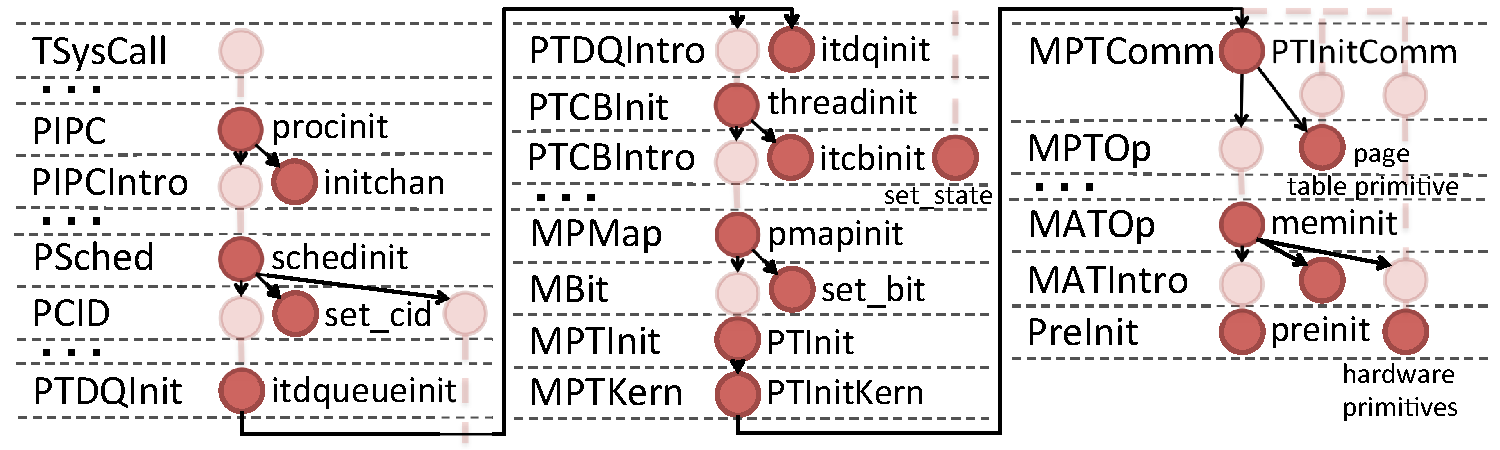
\includegraphics[scale=0.3]{figs/initialization}
\caption{Call graph of \mCTOSbase{} initializer}
\label{fig:mcertikos-init-call-graph}
\end{figure}

%\vspace*{-8pt}
\paragraph{\mCTOShyper{}}
The \mCTOShyper{} kernel provides core primitives to build
full-fledged user-level hypervisors by supporting one of the two
popular hardware virtualization technologies -- AMD SVM.  The primitives
include the operations for manipulating the virtual machine status,
handling VMEXITs, starting or stopping a virtual machine, {\it etc}.
The details of virtualization, e.g., the virtual machine control block
and the nested page table, are hidden from the guest applications.
The hypervisor functionalities are implemented in nine layers and then
inserted in between process management and interrupt handling layers.
The layered approach allows us to do so while (1) only modeling
virtualization-specific structures when needed; (2) retaining
primitives in the layer interface \textsf{PProc} by systematic lifting; and
(3) adding new primitives (including a new initialization function)
guaranteed not to interfere with existing primitives.

%\vspace*{-8pt}
\paragraph{\mCTOSringz{}}
The \mCTOSringz{} kernel explores a different dimension---instead
of adding intermediate layers, we augmented a few existing layers 
(in \mCTOShyper{}) with support of ring 0 processes.
The main modification is at
\textsf{PProc}, where an additional kind of threads is defined.
However, all the layers between \textsf{PProc} and \textsf{TSysCall} also
need to be extended to expose the functionality as system calls.
Thankfully, since all the new primitives are already described in deep
specifications, lifting them to system calls only requires equality
reasoning in Coq.

%\vspace*{-8pt}
\paragraph{\mCTOSembed{}}
The \mCTOSembed{} kernel cuts features down to a bare minimum: it does
not switch to user mode, hence does not require memory protection and
does not provide system call interfaces.  This requires \emph{removing}
features instead of adding them.  Since the layered structure minimizes
entanglements by eliminating unnecessary dependencies and code coupling,
the removal process was relatively easy and straightforward.
Moreover, removing the top 12 layers requires no additional
specifications for those now top-level primitives---deep specifications
are suitable for both internal reasonings and external descriptions.  Thread and process
management layers now sit directly on top of physical memory
management; virtual memory is never enabled.  The
layers remain largely the same barring the removal of primitives
mentioning page tables.}


